\documentclass[utf-8]{ctexart}


\usepackage{graphicx}
\usepackage{listings}
\usepackage{xcolor}

\lstset{
  language={[ANSI]C},
  keywordstyle=\color{blue!70},
  basicstyle=\small,
  commentstyle=\color{red!50!green!50!blue!50},
  frame=none,
  breakautoindent=true,
  rulesepcolor=\color{red!20!green!20!blue!20},
  showstringspaces=false,
  numbers=left,
  breaklines=true
}
\begin{document}
\title{hihoCoder笔记}
\author{AbnerZheng}
\date{2016/08/25}
\maketitle{}
\begin{abstract}
  知道hihoCoder这个网站,大概是15年九月份校招的时候,当时Line和微软就是采用这个
  OA系统,体验很一般,当时并没有太多的印象。后面发现他每周都有一个hiho一下,已经做了
  一百多期了,就稍稍体验了把,感觉非常不错。前面的几十周,有教学提示,题目安排统
  一而有序,感觉非常适合我,然后就想着每天中午都刷刷题,做做笔记,希望自己的算法
  能力能有较大的提升。
\end{abstract}

\section{第十周-后序遍历}
\label{sec:week_10}

\subsection{题解}
\label{sec:week_10_ana}

这题是已知前序和中序遍历,求后序遍历。在二叉树还原中,通过两个遍历得到另一个遍历,
有一个结论是中序遍历必须存在。

对于一个二叉树,如下:

\vspace{\doublerulesep}

\begin{center}
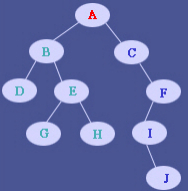
\includegraphics[width=.5\textwidth]{../images/note/binary_tree.jpg}
\end{center}


其前序遍历为: ABDEGHCFIG
其后序遍历为: DBGEHACIJF
由前中后序遍历的定义, 有
\begin{eqnarray}
pre(T)  &=& T +  pre(T.leftChildren) + pre(T.rightChildren)\\
 in(T)  &=& in(T.leftChildren) + T + in(T.rightChildren)   \\
post(T) &=& post(T.leftChildren)+post(T.rightChildren) + T
\end{eqnarray}
现在已知前序和中序遍历,现求解
\begin{eqnarray*}
  post(pre(T), in(T))  &=& post(pre(T.leftChildren), in(T.leftChildren)) + \\
                       & & post(pre(T.rightChildren), in(T.rightChildren)) + T \\
\end{eqnarray*}
所以关键的地方在于找到如何划分前序和中序遍历。因为子树大小相同,那么对于子树的前
中后序的长度是一致的, 根据这一条件,可以很方面地得到这些划分。代码如下:

\begin{lstlisting}
void post(string pre, string in){
    int pos = 0;
    int len_pre = pre.length();
    int len_in = in.length();
    if(len_in == 0){
        return;
    }

    string::iterator iter;
    for(iter = in.begin(); iter!=in.end(); ++iter){
        if(*iter == pre[0]){
            break;
        } else{
            ++pos;
        }
    }

    /**
      in(0,(pos-1)) -> in.leftChild ->  len(in.leftChild) = pos
      in(pos) -> T
      in(pos+1, len(in)-1) -> in.rightChild -> len(in.rightChild) = len(in) - (pos+1)
    */

    int len_left = pos;
    int len_right =  len_pre - pos -1;

    post(pre.substr(1, len_left), in.substr(0,len_left));
    post(pre.substr(pos+1,len_right), in.substr(pos+1,len_right));
    cout<< pre[0];
}
\end{lstlisting}

\section{第十一周-树的最长路径}
\label{sec:week_11}
这题是 bn

\end{document}
